\makeatletter
\makeatother
\documentclass[10pt,english]{article}\usepackage{graphicx, color}
%% maxwidth is the original width if it is less than linewidth
%% otherwise use linewidth (to make sure the graphics do not exceed the margin)
\usepackage{alltt}
\usepackage[T1]{fontenc}
\usepackage[latin9]{inputenc}
\usepackage{geometry}
\geometry{left=1.5cm,right=1.5cm,top=2cm,bottom=2cm}
\usepackage{fancyhdr}
\pagestyle{fancy}
\setlength{\parskip}{\smallskipamount}
\setlength{\parindent}{0pt}
\usepackage{amsthm}
\usepackage{amsmath}

\makeatletter

%%%%%%%%%%%%%%%%%%%%%%%%%%%%%% LyX specific LaTeX commands.
\providecommand{\LyX}{L\kern-.1667em\lower.25em\hbox{Y}\kern-.125emX\@}

%%%%%%%%%%%%%%%%%%%%%%%%%%%%%% Textclass specific LaTeX commands.
\numberwithin{equation}{section}
\numberwithin{figure}{section}

\@ifundefined{date}{}{\date{}}
%%%%%%%%%%%%%%%%%%%%%%%%%%%%%% User specified LaTeX commands.
\pagestyle{empty} 

\makeatother

\usepackage{babel}
\begin{document}

\title{Sample Task - Ratio Analysis\\
Report}


\author{Xiaohui Li, Yuxin Ma}

\maketitle


In order to make more further discussion, at first for the preliminary work, we modified our function to make it much more general, \emph{RatioPower}, including the situation of homoscedasticity or heteroscedasticity for the variance level, minimum, maximum, median or mean for the ratio level, and uniform distribution or log-normal distribution for the another variance level.

\section{Homoscedasticity}

Firstly, we consider that $\sigma_k$ has the same variance, which is a homoscedasticity case. We define $r_1=\frac{Y_1}{\sigma_1}$ and $r_k=\frac{\sigma_k}{\sigma_1}$. And we generate $\sigma_k$ by $Y_1$, $r_1$ and $\sigma_1$. Then we do a 100$\times$20 times test where the scaling of $r_1$ varies from 0 to 2 and the scaling of $r_k$ varies from 0 to 10. We get the plot as follow.
\begin{figure}[htbp]
\centering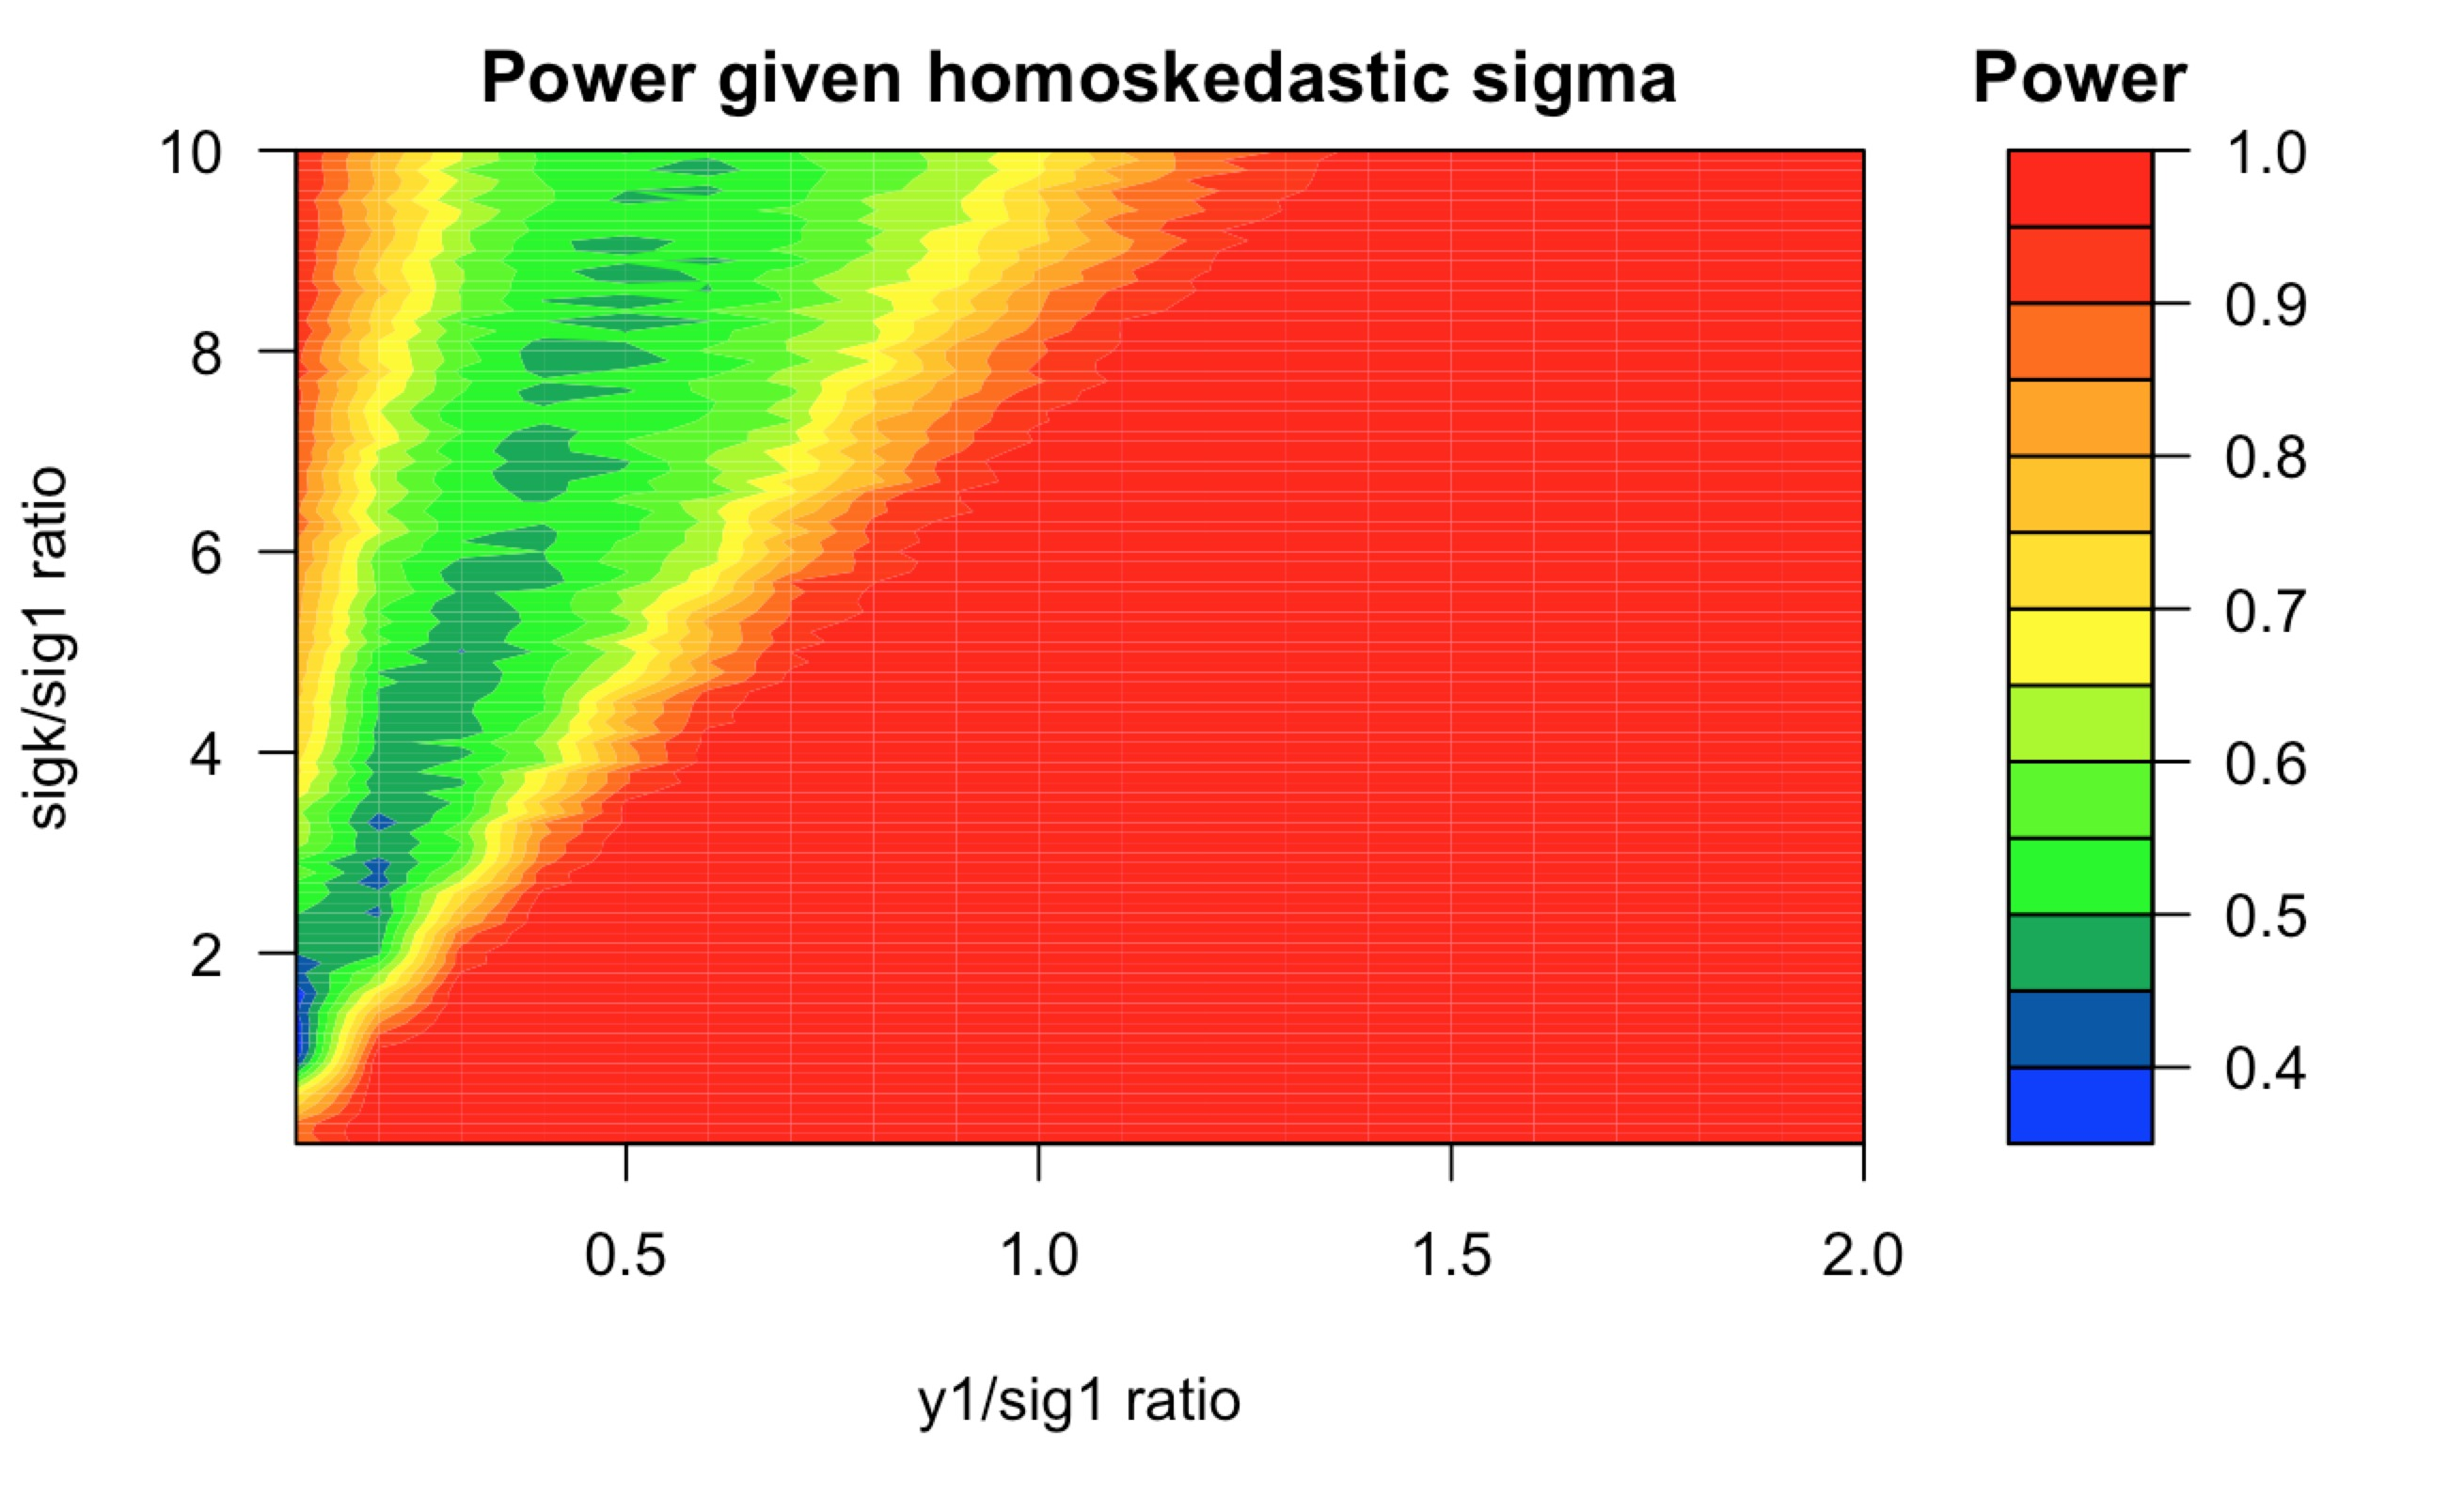
\includegraphics[width=6.5in,height=4in]{homo}
\caption{Homoscedasticity with $r_1$ varying from 0 to 2}
\end{figure}

We can see that there is an increasing linear trend as $\sigma_1$ and $\sigma_k$ increase and the power converges to 1, the increasing trend starts from a ratio $\frac{r_k}{r_1}$ of around 20, which is "blue shade". Also we can see that if $\sigma_1$ takes very large values, the power will always be 1 and we will always reject to the null hypothesis, which does not have such significant results.

\section{Heteroscedasticity}
\subsection{Random $\sigma_k$}
This time, we assume the rest  $\sigma_k$s are log-normal distributed and we generate them by the normal distribution with the mean equals to $\log(r_k\cdot Y_1/r_1)$ and take its exponential value. Also we do a 50$\times$20$\times$20 times test where the scaling of $r_1$ varies from 0 to 2 and the scaling of $r_k$ varies from 0 to 10. We plot its power and get a plot having a similar trend as the homoscedasticity case does.
\begin{figure}[htbp]
\centering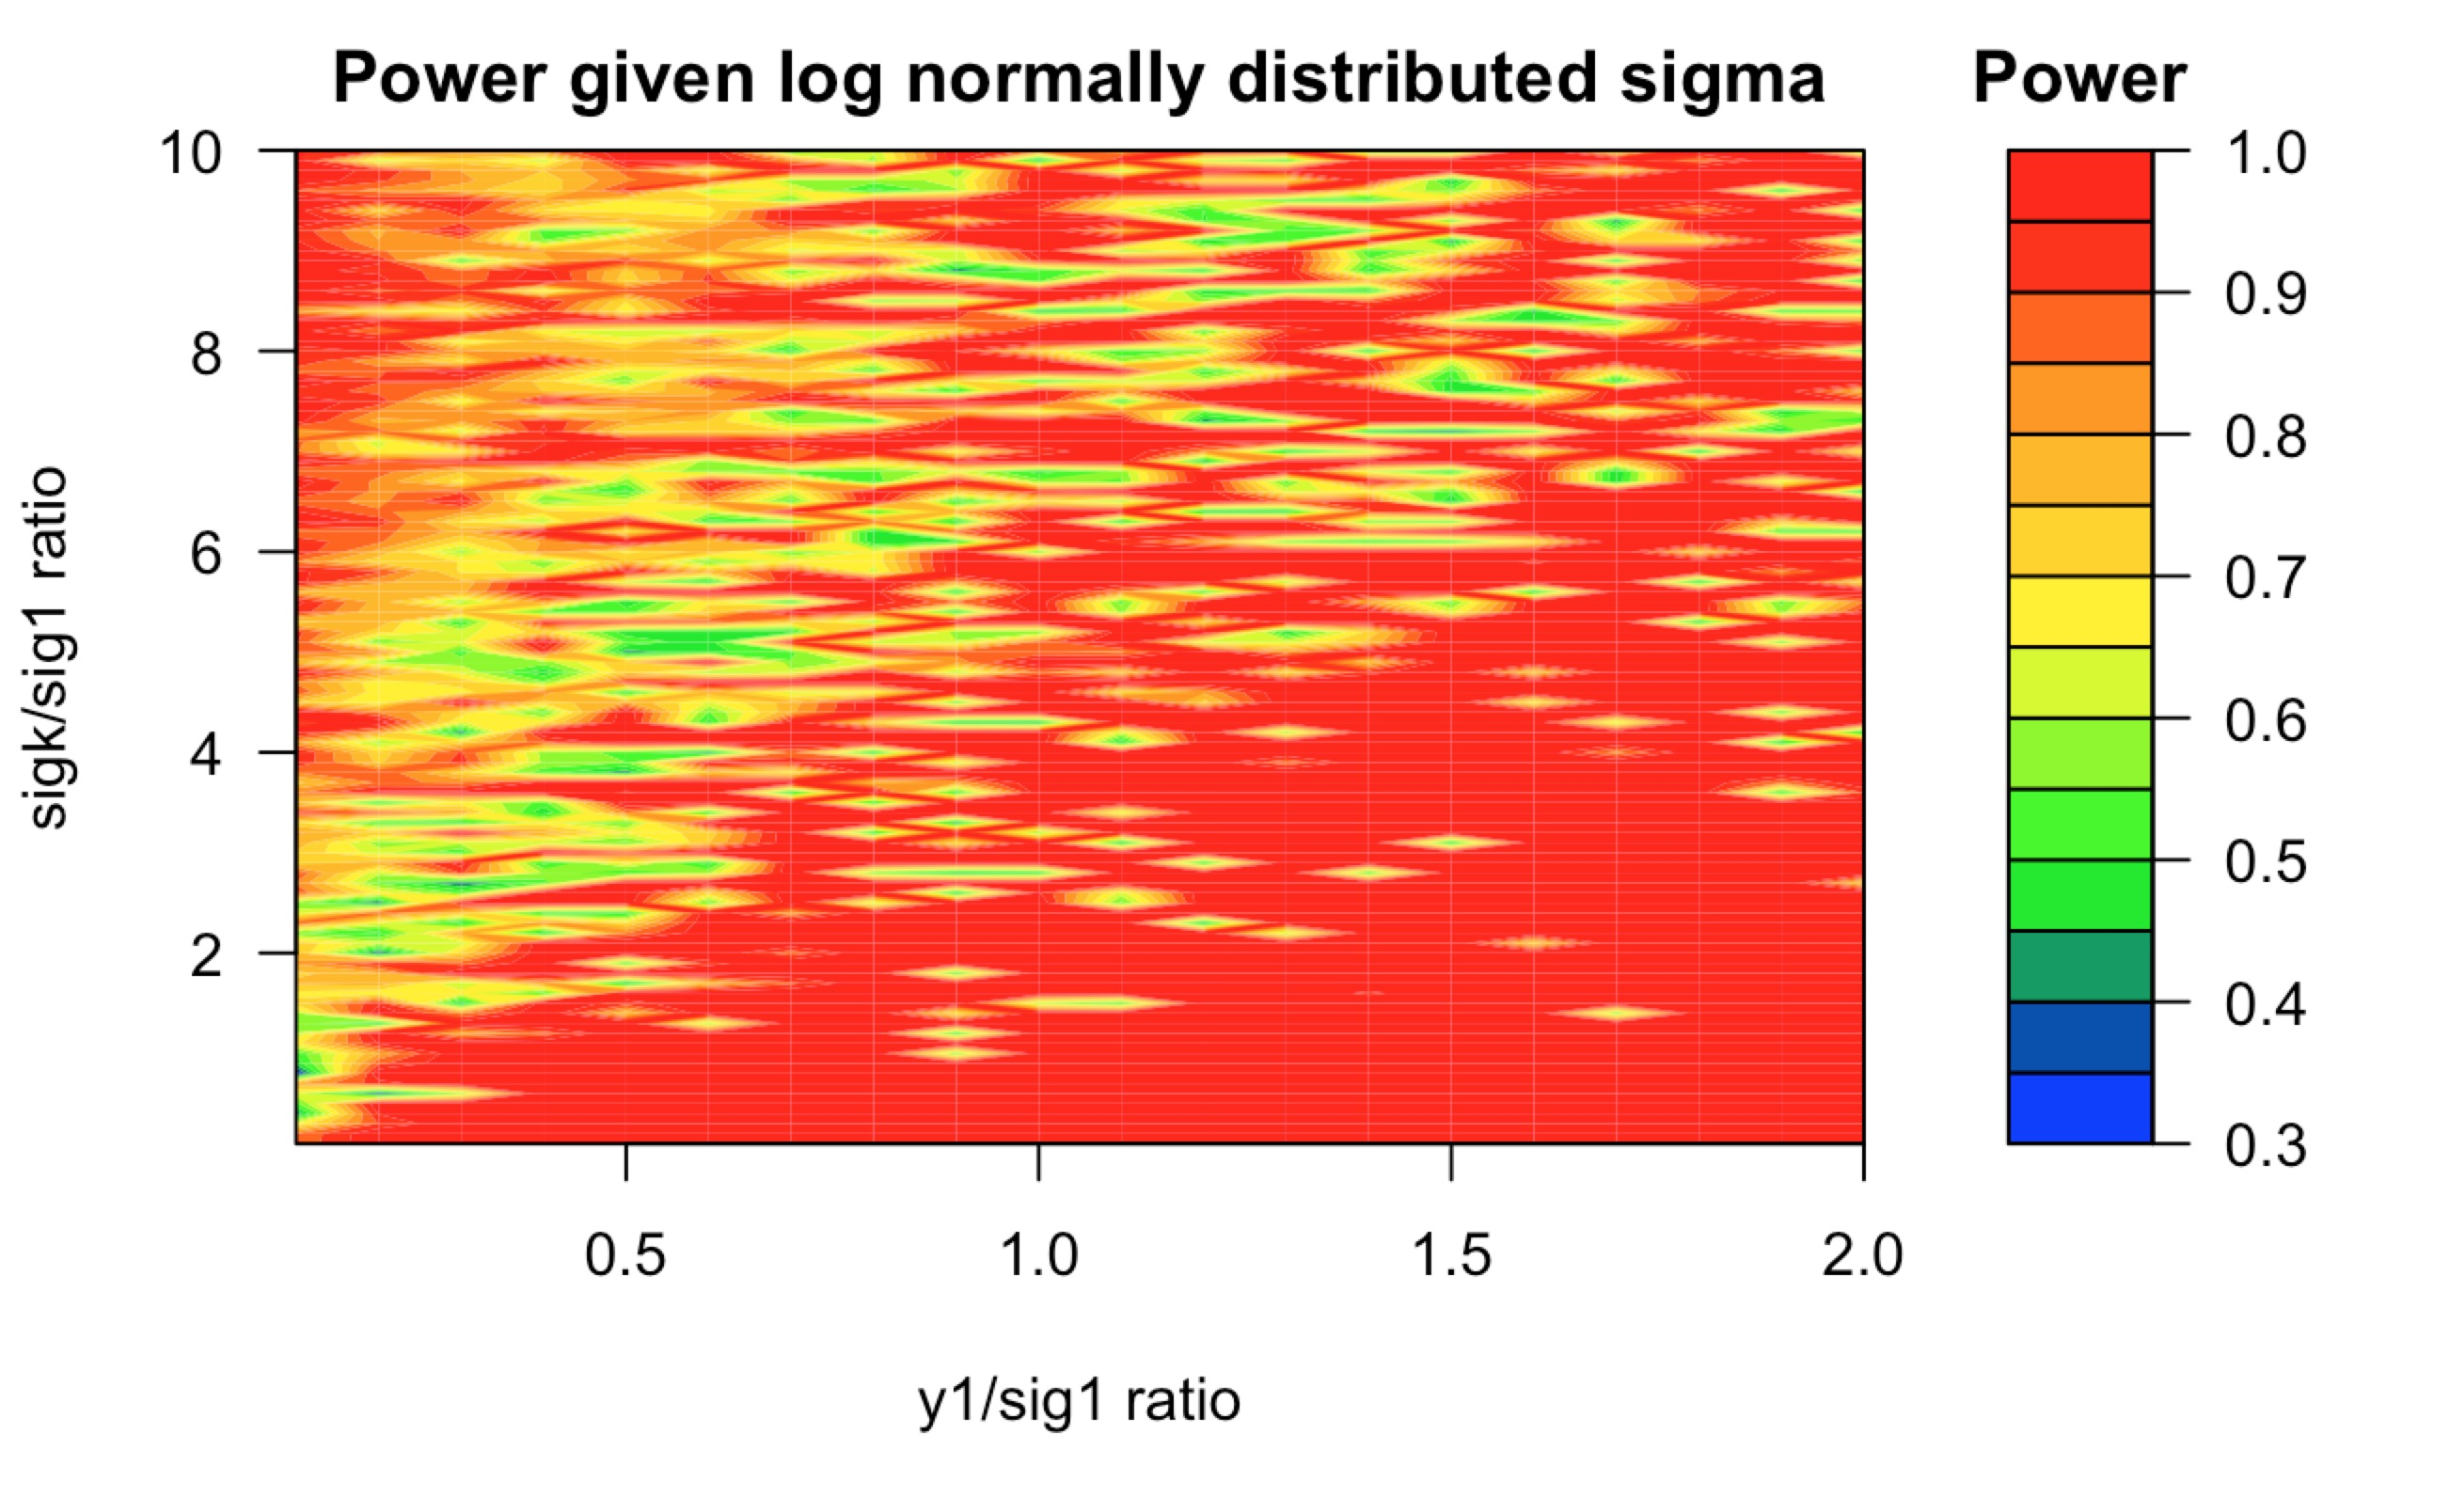
\includegraphics[width=4.5in,height=3in]{hetero}
\caption{Heteroscedasticity}
\end{figure}

As it is depicted in the figure, there is still an "sparsely" increasing linear trend. But compared it with the homoscedasticity case, we can see that it is more discrete and fluctuates around the trend.

\subsection{Random $r_k$}
Unlike previous tests where we generate $r_k$ by the iteration of equidistant increasing, this time we directly generate the random $r_k$ by the uniform distribution or normal distribution to make our tests more general. And for the plot part, we choose a variety of ordinate form, including the minimum, maximum, median and mean of $r_k$.

\subsubsection{Uniform Distribution - Minimum}
We choose $r_1$ varies from 0 to 2. And we generate $r_k$ by the uniform distribution ranging from 0 to 10. Then we choose the minimum of $r_k$ to plot the power as Figure \ref{1}.
\begin{figure}[htbp]
\centering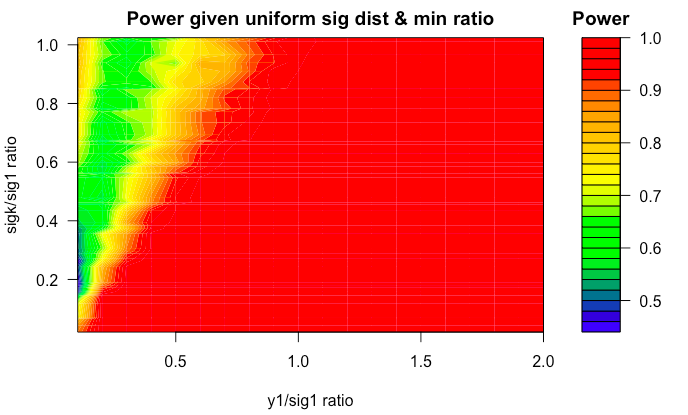
\includegraphics[width=4.5in,height=3in]{uni_min}
\caption{\label{1}Uniform Distribution - Minimum}
\end{figure}
\quad\\
\quad\\
\quad\\
\quad\\
\quad\\
\quad\\
\quad\\
\quad\\
\quad\\
\quad\\
\quad\\
\quad\\

\subsubsection{Normal Distribution - Minimum}
We choose $r_1$ varies from 0 to 2. And we generate $r_k$ by the normal distribution with its mean varying from 0 to 5 and variance equaling to 1 (default). Then we choose the minimum of $r_k$ to plot the power as Figure \ref{2}.
\begin{figure}[htbp]
\centering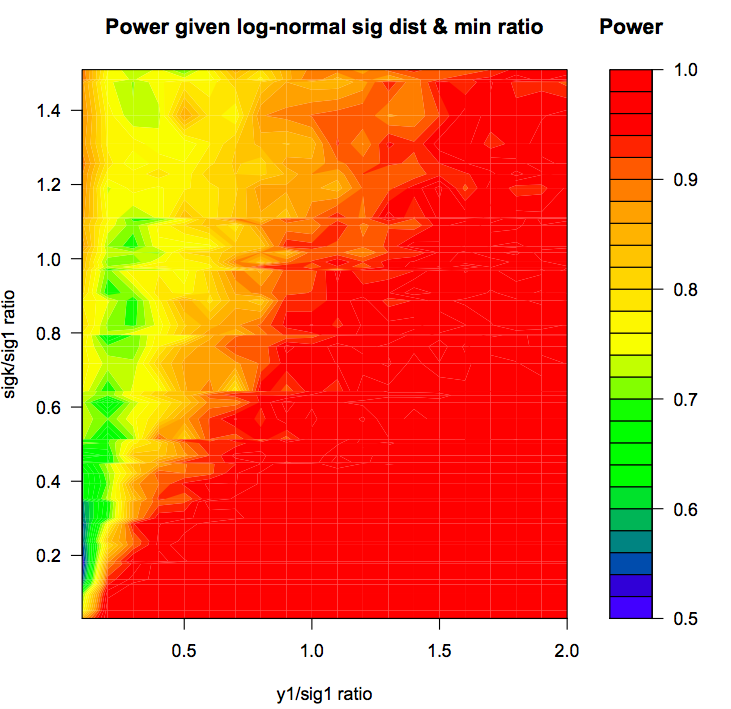
\includegraphics[width=4.5in,height=3in]{ln_min}
\caption{\label{2}Normal Distribution - Minimum}
\end{figure}
\quad\\
\quad\\
\quad\\
\quad\\
\quad\\
\quad\\

\subsubsection{Normal Distribution - Maximum}
We choose $r_1$ varies from 0 to 2. And we generate $r_k$ by the normal distribution with its mean varying from 0 to 5 and variance equaling to 1 (default). Then we choose the maximum of $r_k$ to plot the power as Figure \ref{3}.
\begin{figure}[htbp]
\centering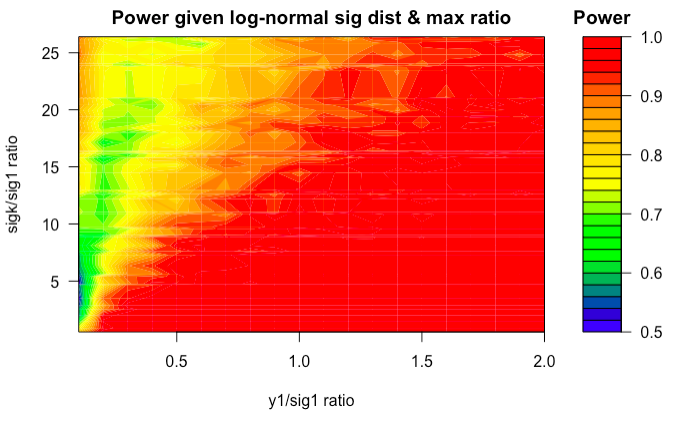
\includegraphics[width=4.5in,height=3in]{max}
\caption{\label{3}Normal Distribution - Maximum}
\end{figure}

\subsubsection{Normal Distribution - Median}
We choose $r_1$ varies from 0 to 2. And we generate $r_k$ by the normal distribution with its mean varying from 0 to 5 and variance equaling to 1 (default). Then we choose the median of $r_k$ to plot the power as Figure \ref{4}.
\begin{figure}[htbp]
\centering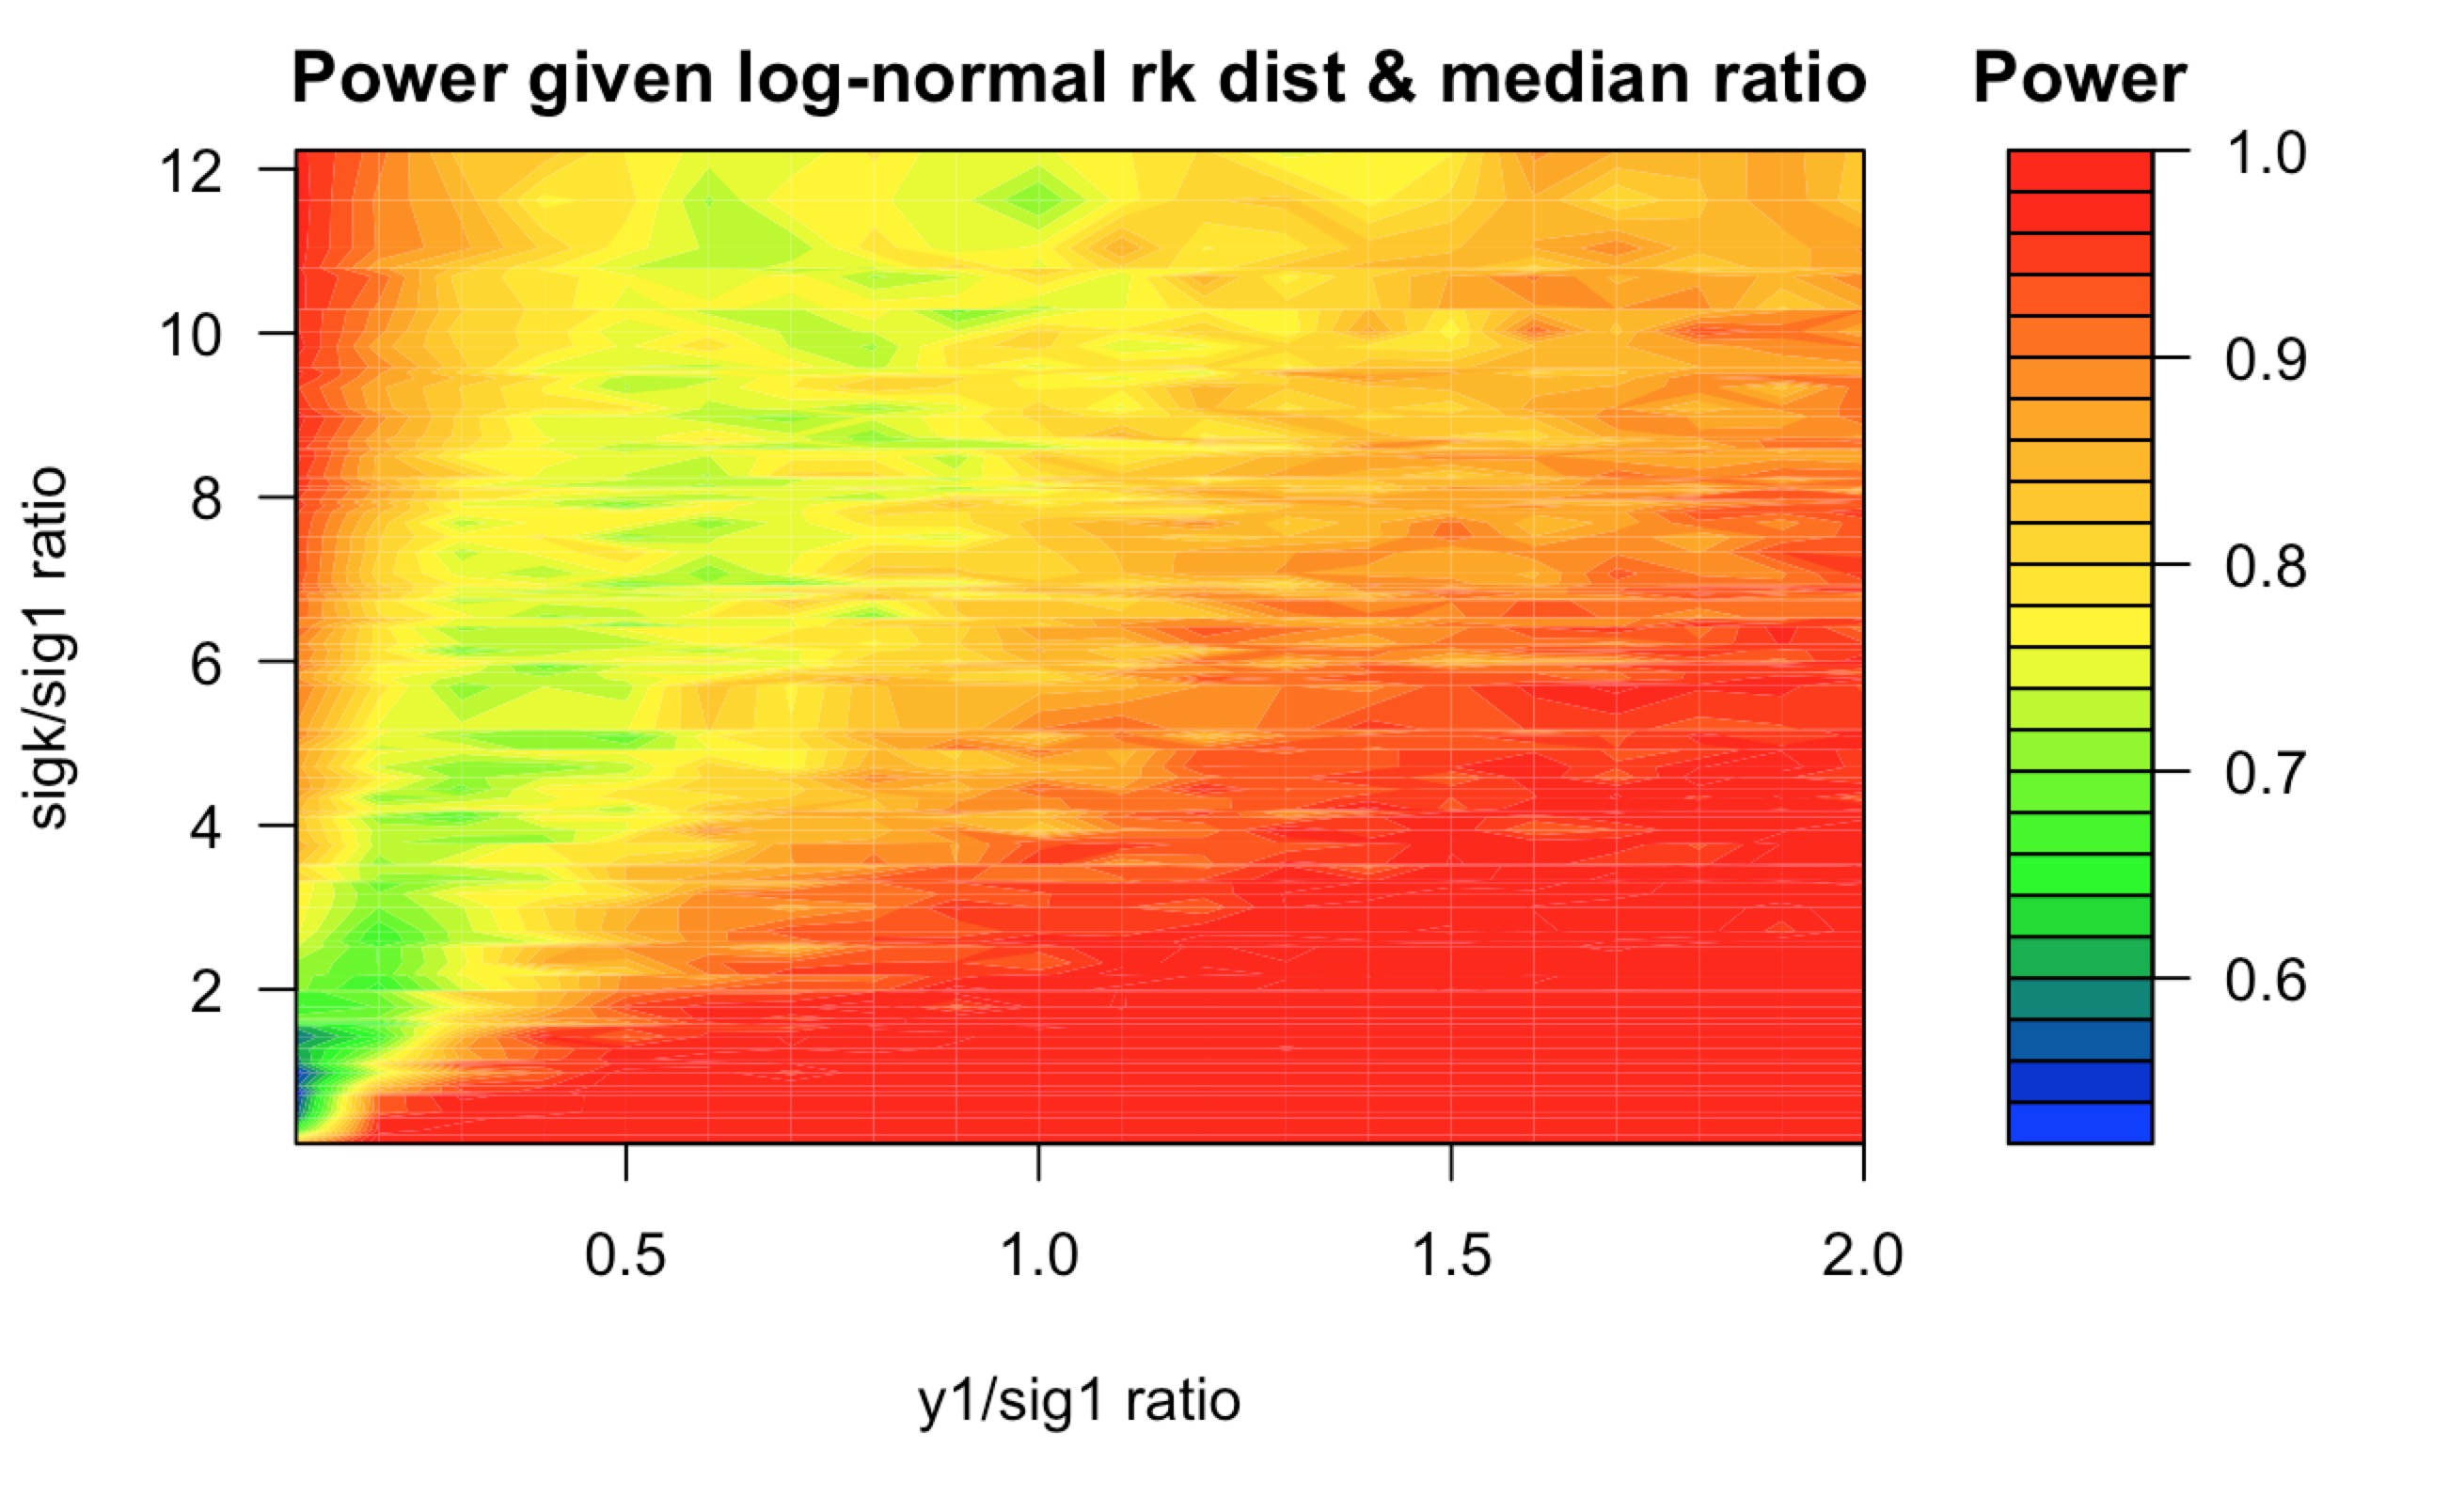
\includegraphics[width=4.5in,height=3in]{med}
\caption{\label{4}Normal Distribution - Median}
\end{figure}

\subsubsection{Normal Distribution - Mean}
We choose $r_1$ varies from 0 to 2. And we generate $r_k$ by the normal distribution with its mean varying from 0 to 5 and variance equaling to 1 (default). Then we choose the mean of $r_k$ to plot the power as Figure \ref{5}.
\begin{figure}[htbp]
\centering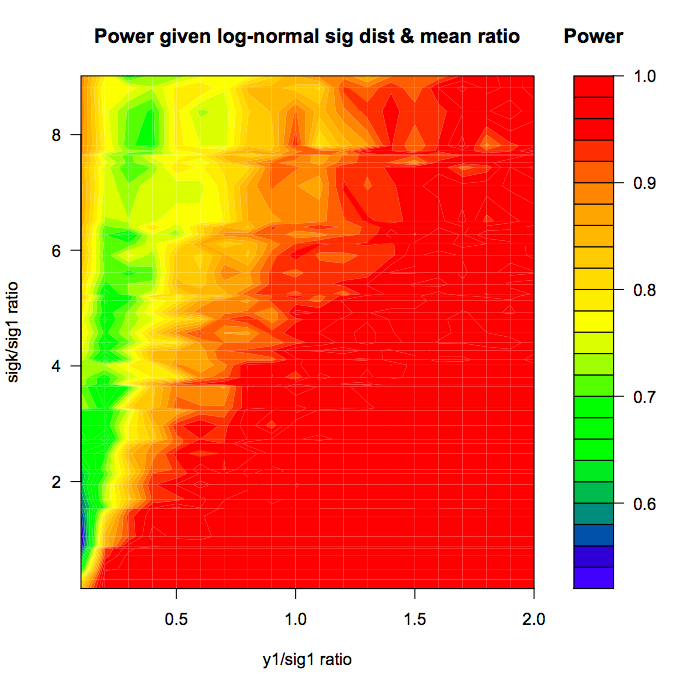
\includegraphics[width=4.5in,height=3in]{men}
\caption{\label{5}Normal Distribution - Mean}
\end{figure}

\subsection{Conclusions of Random $r_k$}
We can see that when we take the random $r_k$, for either uniform or normal distribution, it will always have a increasing trend like the homoscedasticity case and the heteroscedasticity case for random $\sigma_k$. But it is obvious that the power of the uniform distribution increases much more regularly and steadily, unlike the normal distribution, which will be more discrete. But in total, we can see that the general trend is evident as depicted in contour plots.\\
\quad\\
Specifically, we could find that given the $r_k \sim\log{\text{-Normal}}$ assumption, the power increasing more than $\sigma_k$ log-normal. While the normal-median case is a special case where the power increase slowly. Given fixed $r_k = \frac{\sigma_k}{\sigma_1}$, as $r_1 = \frac{\bar{Y_1}}{\sigma_1}$  increases, the power increase, while given fixed $r_1 = \frac{\bar{Y_1}}{\sigma_1}$, as $r_k = \frac{\sigma_k}{\sigma_1}$  increases, the power decreases. The power converges to 1 with increase of $r_1 = \frac{\bar{Y_1}}{\sigma_1}$.

\end{document}










